\section{Communications Subsystem}
The communications system that was decided upon consists of a RFD 900+ transceiver that is linked to a ground station and other satellites with the same chip. The transceiver chip is connected to two antennas that increase gain allowing for larger uplink and downlink margins. The chip communicates to the OBC via UART and for a simple two node communication system works out of the box. For recovery purposes it was decided the satellites to be launched at the same time as SnapSat will be linked together via a multipoint network. 

\noindent
The requirements of the communication system include emitting a beacon containing the whole orbit data (WOD) collected every 30 seconds. IT must also be able to accept commands from the ground station and send back payload data to earth. An example of the commands this system is able to receive and execute are turning transmissions on and off to control which satellite is emitting at a set time.

\subsection{Componenets}
\begin{figure}[H]
    \centering
    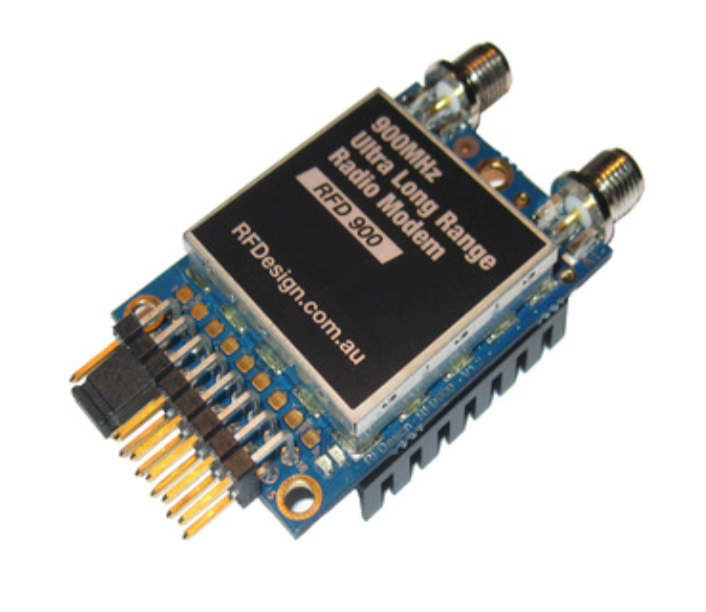
\includegraphics[width=0.6\linewidth]{./figures/rfd}
    \caption{RFD900}
\end{figure}
\noindent
As mentioned above the core of the communications subsystem is the RFD 900+ transceiver from RFDesigns. It was decided that the Arduino shield used to interface the transceiver with the OBC was not necessary and direct soldering on to our PCBs would allow for a more compact design. To complete this the following pins were connected to the associated Arduino pins with data in from the transceiver connecting to data out of the Arduino and vice versa. 
\begin{figure}[H]
\centering
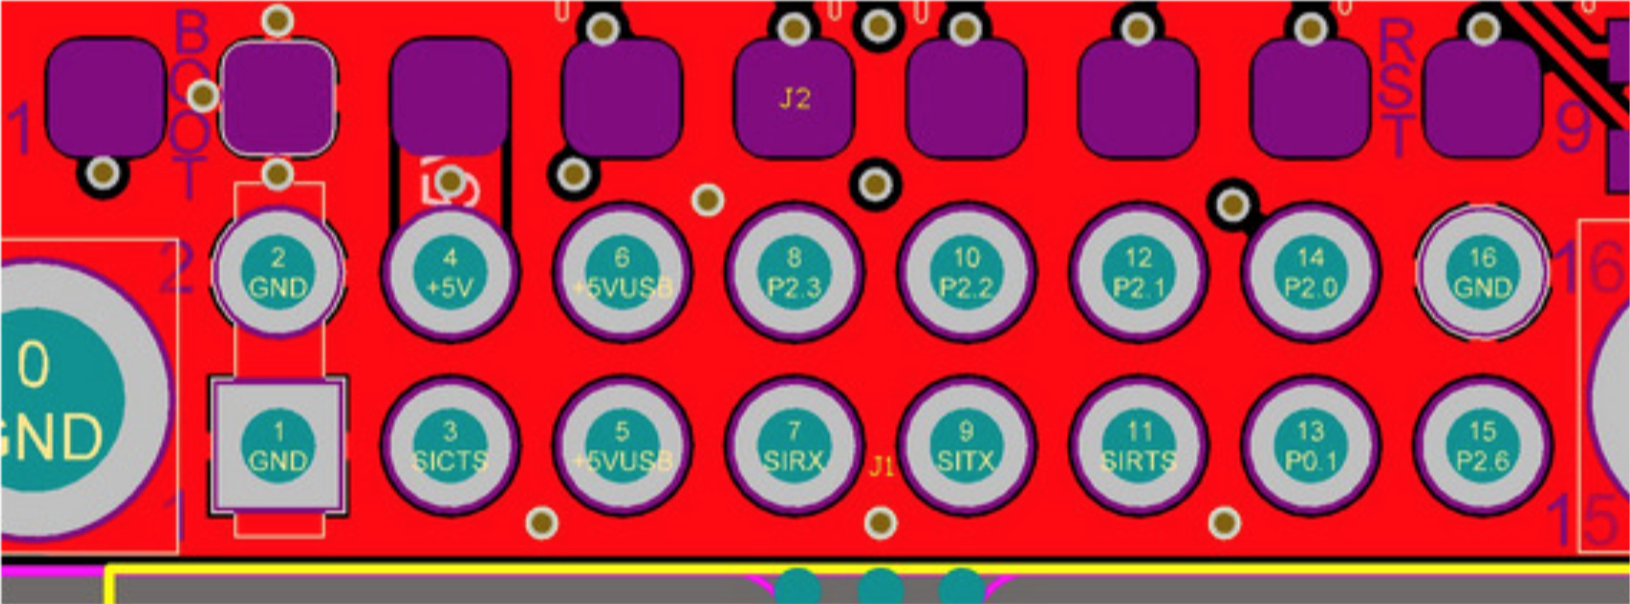
\includegraphics[width=\linewidth]{./figures/pins}
\caption{Pin Diagram}
\end{figure}
\begin{figure}[H]
    \centering
    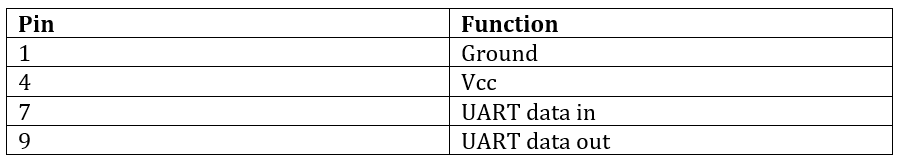
\includegraphics[width=0.75\linewidth]{./figures/tablepins}
    \caption{Table of pins used}
\end{figure}
\noindent
The transceiver has a wide range of settings that can be customised for different missions and because of this is used extensively in balloon launches. The data rate ranges from 4 Kbits/s to 250 Kbits/s and this can be set or dynamically change depending on the signal. The line of sight range that will be utilised has been recorded between 40km – 60km, making it ideal for a balloon launch which normally ascends to 30km. An air speed of 64kps will give a range of about 40km depending on antenna. If the air speed is set to be lower, the range of the wireless link increases but the amount of data that you can send will be limited. 
\begin{figure}[H]
    \centering
    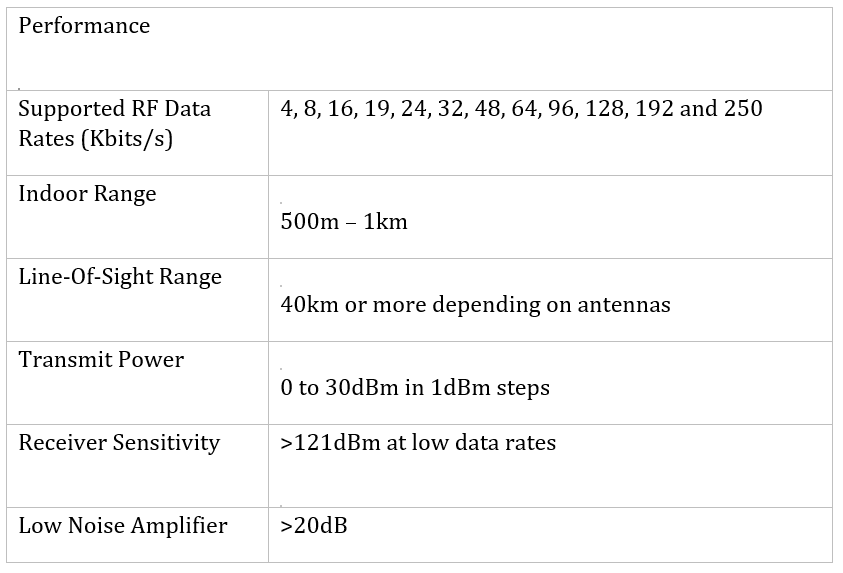
\includegraphics[width=0.9\linewidth]{./figures/performance}
\end{figure}
\noindent
The RFD900+ operates within the frequency band of 902 MHz-928MHz and uses frequency hopping spread spectrum (FHSS) to improve its immunity to interference. 
\begin{figure}[H]
    \centering
    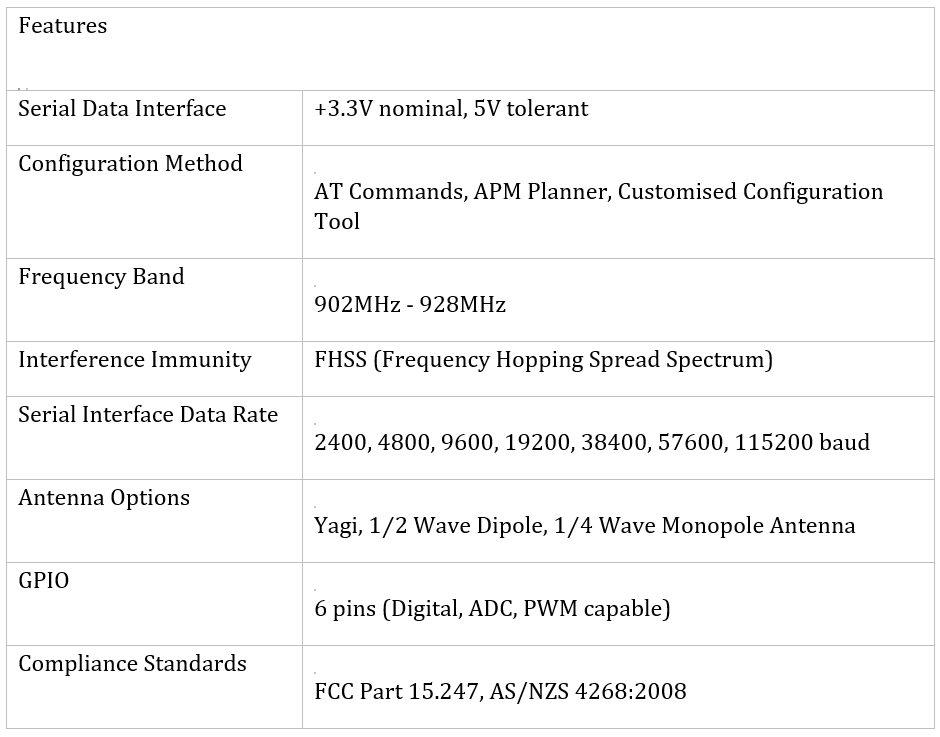
\includegraphics[width=0.9\linewidth]{./figures/features}
\end{figure}
\noindent
The configuration that was chosen includes a baud rate of 57600 with no parity, 8 data bits and 1 stop bit. This was chosen to maximise the data send back to the ground station whilst maintaining a solid link margin.
\begin{figure}[H]
    \centering
    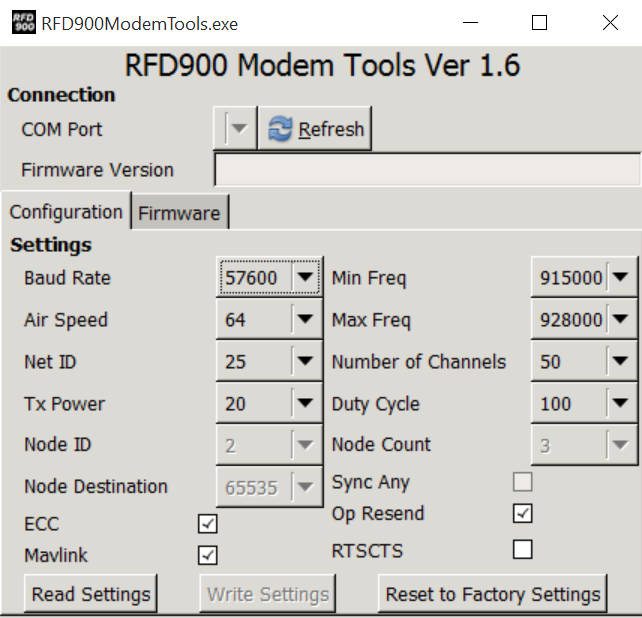
\includegraphics[width=0.75\linewidth]{./figures/rfd2}
    \caption{Settings used with transciever}
\end{figure}
To increase the gain on both ends of the transmission, different antennas will be used at the ground station compared to the satellite. At the ground station we will utilise a yagi antenna. Yagi antennas are recommended for Ground-Station applications due to their size. They have approximately 6dBi gain and give significant link budget improvement when compared to standard dipole, or monopole antennas. 
\noindent
On the satellite we will use two quarter wave antennas. The choice was between this and half wave dipole antennas but the quart wave was declared superior due to it’s small size. Quarter Wave Monopole Antennas are recommended for air-borne, or space constrained applications. They are required to be mounted on a ground plane of approximately 20cm diameter or more to operate as intended.
\begin{figure}[H]
    \centering
    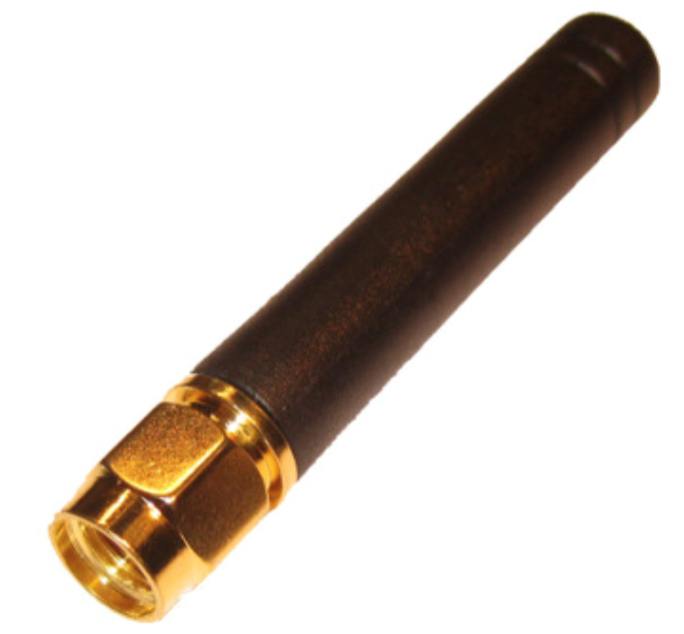
\includegraphics[width=0.6\linewidth]{./figures/antennae}
    \caption{Quarter Wave Monopole Antenna}
\end{figure}
The RFD900 has two antenna ports and firmware which supports diversity operation of antennas. During the receive sequence the modem will check both antennas and select the antenna with the best receive signal. In the case of only one antenna connected, it will automatically select the port with the antenna connected. Testing by Silicon Labs has shown that link budgets can be improved in the order of 6-8dB by employing a diversity scheme.

\noindent 
Polarisation diversity is the case where the antennas are perpendicular to each other. i.e. one vertical, and one horizontal. This is effective in reducing multipath effects which affect one or the other polarisation. We will utilise this principle and set the antennas at a 90-degree angle to each other.

\noindent
The RFD900 can be implemented in either simple pair between two nodes or a multipoint network. In our case we have opted to use the multipoint network to allow the satellites to communicate in the air, relaying their position to aid in recovery. The following is an example of a 5 node network that will be ideally implemented. The network consists of Node 0, the ground station, Node 1, the mother satellite, and the remaining nodes are the other satellites. This structure has not been confirmed as the satellites participating in the launch is yet to be decided.
\begin{figure}[H]
    \centering
    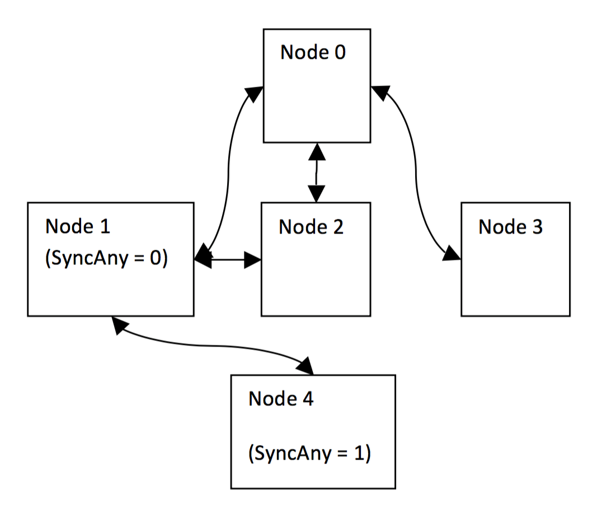
\includegraphics[width=0.7\linewidth]{./figures/nodes}
    \caption{Five-node Network Setup}
\end{figure}

\paragraph{Ground Station}
Mobile ground station utilizing the same model rfd900+ transceiver connected to a yagi antenna. Yagi antennas are recommended for Ground-Station applications due to their size. They have approximately 6dBi gain and give significant link budget improvement when compared to standard dipole, or monopole antennas. 

\noindent
The system has been set up to receive a number of commands from the ground station and act upon them. This allows it to be controlled by an operator and gives it superior functionality. The list of commands is as follows:

\noindent
User Commands
\begin{enumerate}
    \item	SET/GET TRANSMIT ON/OFF - Sets transmit to on or off
    \item	SET/GET MODE [mode]  - Sets the mode of the satellite
    \item	DOWNLOAD PAYLOAD - Download all scientific data that hasn’t been sent yet
    \item	SET PICTURE RATE - Set how often pictures are taken
    \item	SET [variable] [value] - Change the value for specific variables in code
    \item	RESET - Causes the device to reset
    \item	DELETE [date] - delete data before the given date
    
\end{enumerate}

\subsection{Link Budget Summary}
After calculating the link budget for the satellite in orbit we now have a much larger factor of safety as the free space path loss is reduced by 21 dB to 101 dB, giving us a larger margin, even considering the change in transceiver. The RFD 900+ has been used numerous times successfully for balloon launch, thereby confirming the margin is adequate. The assumptions made with the link budget include clear sky with normal humidity and a temperature of 30 degrees Celsius.
\begin{figure}[H]
    \centering
    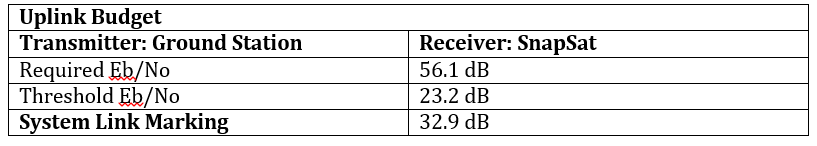
\includegraphics[width=\linewidth]{./figures/uplink}
    \caption{Uplink budget}
\end{figure}
\begin{figure}[H]
    \centering
    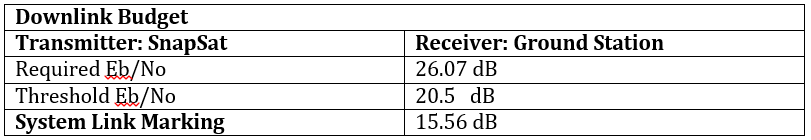
\includegraphics[width=\linewidth]{./figures/downlink}
    \caption{Downlink budget}
\end{figure}